%\documentclass[preprint, review, 3p, authoryear]{elsarticle}
\documentclass[10pt, a4paper]{article}

%\usepackage{setspace}
\usepackage[utf8]{inputenc}
\usepackage{amsmath, amssymb, amsthm, bbm}
\usepackage{xcolor}
\usepackage{graphicx}
\usepackage[authoryear]{natbib}
\usepackage{apalike}
\usepackage{relsize}
\usepackage{array}
\usepackage{multirow}
\usepackage{showlabels}
\usepackage{setspace}

%Add line numbering
%Line numbering can be incorporated by using the lineno package. Add these statements in the preamble:
\usepackage{lineno}
\linenumbers

\DeclareMathOperator*{\argmax}{arg\,max}

\newtheorem{prob}{Problem}
\newtheorem{prop}{Proposition}
\newtheorem{definition}{Definition}

%%%%% bold symbol in math enviornment
\newcommand{\m}[1]{\boldsymbol{#1}}

\title{Merging the components of a finite mixture using  posterior probabilities}
\author{M. Comas-Cufí \and J.A. Martín-Fernández \and G. Mateu-Figueras}

%\doublespacing
\begin{document}

\begin{spacing}{1.9}

\pagenumbering{arabic}

\maketitle

\section{Introduction}

%Cl
The most standard parametric approach in cluster analysis assumes data can be modelled by a \emph{finite mixture of distributions} (FM){\color{blue} Martin: cal investigar si altres articles fan servir acrònim i quin? jo he posat FM però no estic gens segur..}. A FM is a probability distribution with probability density function (pdf) defined as the linear combination of pdf from other probability distributions defined in $\mathbb{X}$, the sample space. In general, the pdf $f$ of a FM is
\begin{equation}\label{mixt}
f(\;\cdot\; ; \pi_1, \dots, \pi_k, \m\theta_1, \dots, \m\theta_k) = \pi_1 f_1(\;\cdot\; ; \m\theta_1) + \dots + \pi_k f_k(\;\cdot\; ; \m\theta_k),
\end{equation}
where $\m\theta_1, \dots,  \m\theta_k$ are the parameters of the pdf $f_1, \dots, f_k$ respectively and, because $\int_{\mathbb{X}}f = 1$ the restriction $\sum_{\ell = 1}^k \pi_\ell = 1$ holds. The pdf $f_1, \dots, f_k$ are called the \emph{components} of the FM, or simply the \emph{mixture components}.


When model-based clustering is based on a FM, a common approach consist of two steps {\color{blue} Martin: per aquí cal dir alguna cosa del valor de k}:
\begin{enumerate}
\item to find a suitable estimators $\hat{\pi}_1, \dots, \hat{\pi}_k,$ $\hat{\m\theta}_1, \dots, \hat{\m\theta}_k$ of parameters $\pi_1, \dots, \pi_k,$ $\m\theta_1, \dots, \m\theta_k$, and
\item to classify each observation according to the maximum posteriori criteria, i.e., one observation $\m x_i \in \mathbb{X}$ is classified to cluster $c$ if and only if
\[
c=\argmax_{j=1}^k \frac{ \hat{\pi}_j f_j(\m x_i ; \hat{\m\theta}_j) }{\sum_{\ell=1}^k \hat{\pi}_\ell f_\ell(\m x_i ; \hat{\m\theta}_\ell) }.
\]
\end{enumerate}


\cite{lee2004combining,hennig2010methods,baudry2010combining,melnykov2013distribution,pastore2013merging} noted that associating one mixture component to one cluster can be misleading, because different mixture components can be not separated enough to be considered as a unique cluster. Instead, they proposed that one cluster can be formed by the combination of different mixture components. Therefore, one crucial point of this clustering method is how to decide which components have to be merged, the focus of this article.

Once the criterion for merging component is adopted, the common procedure to make the final clustering from the initial FM is a hierarchical combination of components, that is, a hierarchical sequence of \emph{partitions}. A partition $\mathcal{P}_s=\{ I_1, \dots, I_s\}$ of $\{1, \dots, k\}$ is a set of subsets $I_p$ of $\{1, \dots, k\}$, called $parts$, such that $\bigcup_{I_p \in \mathcal{P}_s} I_p = \{1, \dots, k\}$ and for all two parts $I_p, I_j \in \mathcal{P}_s$, $I_p \cap I_j = \emptyset$ holds. Importantly, the pdf $f$ of a FM (Eq.~\ref{mixt}) can be rewritten as
\begin{equation}
f = \pi_{I_1} f_{I_1} + \dots + \pi_{I_s} f_{I_s},
\label{mixt_part}
\end{equation}
where $f_{I_p} = \sum_{j \in I_p} \frac{\pi_j}{\pi_{I_p}} f_j(\;\cdot\; ; \m\theta_j)$ and $\pi_{I_p} = \sum_{\ell \in I_p} \pi_\ell$. A hierarchical sequence of partitions $\mathcal{P}_1, \dots, \mathcal{P}_k$ of $\{1,...,k\}$, verifies that
  
\begin{itemize}
\item $\mathcal{P}_1$ is the one-part partition $\mathcal{P}_1 = \{ \{1, \dots, k\} \}$,
\item for each $s$, $1 <  s \leq k$, $\mathcal{P}_{s}$ has $s$ elements,
\item if a part $I_p \in \mathcal{P}_{s-1}$ then either there is a part $I_a \in \mathcal{P}_{s}$ with $I_p = I_a$ or there are two parts $I_a, I_b \in \mathcal{P}_s$ with $I_p = I_a \cup I_b$, and
\item $\mathcal{P}_k= \{ \{1\},\{2\}, \dots, \{k\} \}$.
\end{itemize}

One can express the posterior probabilities in terms of the partitions. Indeed, let $\rm X = \{\m x_1,\dots, \m x_n\}$ be a sample defined in $\mathbb{X}$. Given a partition $\mathcal{P}_s = \{ I_1, \dots, I_s \}$ the posterior probability of $\m x_i$ being classified to $I_p\in \mathcal{P}_{s}$ is
\[
\hat{\tau}_{i I_p} =  \frac{ \hat{\pi}_{I_p} \hat{f}_{I_p}(\m x_i) }{\sum_{\ell=1}^s \hat{\pi}_{I_\ell} \hat{f}_{I_\ell}(\m x_i)},
\]
and, for a partition  $\mathcal{P}_s$, we define the posterior probability vector as
\[
\hat{\m\tau}_{i \mathcal{P}_s} = \left( \hat{\tau}_{i I_1} , \dots, \hat{\tau}_{i I_s}  \right).
\]
Note that because of $\mathcal{P}_s$ is a partition, $\sum_{p=1}^s \hat{\tau}_{i I_p} = 1$ for $1 \leq i \leq n$.
Moreover, $\m x_i \in \rm X$ is classified to the cluster $c$ if and only if
\begin{equation}\label{cluster_criteria}
c= \argmax_{p=1}^s \{ \hat{\tau}_{i I_p} \}
\end{equation}


In this paper, we review different approaches that we can find in the literature \citep{baudry2010combining, hennig2010methods} to combine the components of a FM. We introduce new approaches based on the ideas introduced by \cite{longford2014} and inspired on the geometric nature of the posterior probabilities i.e using the log-ratio approach. Importantly, although this approaches have been commonly presented for Gaussian mixtures \citep{longford2014,melnykov2013distribution,hennig2010methods,baudry2010combining}, they can be applied using any other probability distribution mixtures because they are based only on the posterior probabilities vectors $\hat{\m\tau}_{i \mathcal{P}_s}$. This fact, encouraged us to introduce a generic definition where an integrated formulation unifies all these merging methods. In addition, this formulation opens a way to define new methods based on the posterior probabilities.

The paper is organised as follows: In Section~\ref{old_methods}, the approaches by \cite{hennig2010methods} and \cite{baudry2010combining} to obtain a hierarchical combination of components are presented using the new notation also adopted for the new proposals. This new notation is the crucial element for the integrated formulation that unifies the methods. In Section~\ref{comparison} a comparison of the different approaches is done using simulated data sets. Finally, Section~\ref{conclusions} contains the conclusions and final remarks.


\section{Hierarchical combination of components}
\label{old_methods}


\subsection{Approach based on Shannon entropy}

The Shannon entropy of a posterior probability vector $\hat{\m\tau}_{i \mathcal{P}_s} = \left( \hat{\tau}_{i I_1} , \dots, \hat{\tau}_{i I_s}  \right)$ of an observation $x_i$, $1 \leq i \leq n$ is
\[
Ent( \hat{\m \tau}_{i \mathcal{P}_s} ) = - \sum_{j=1}^s \hat{\tau}_{i I_j}  log(\hat{\tau}_{i I_j} ).
\]
$Ent( \hat{\m \tau}_{i \mathcal{P}_s} )$ is a concave function with its maximum at $(\frac{1}{s},\dots,\frac{1}{s})$. In terms of posterior probabilities, the maximum is obtained when the probability of $\m x_i$ being generated by each distributions with pdf $\hat{f}_{I_1}, \dots, \hat{f}_{I_s}$. Due to the fact the maximum is the point with more ``confusion'' between parts, \cite{baudry2010combining} proposed to merge those components, $I_a$ and $I_b$, such that $\sum_{i=1}^n Ent( \hat{\m \tau}_{i \mathcal{P}_{s-1}} )$ is maximum. In other words, their criteria proposes to merge those components that after merging, the sum of the entropy of the resulting posterior probability vectors is maximum. The calculation of the previous criteria depends on the posterior probability of each part $\hat{\tau}_{i I_1}, \dots,\hat{\tau}_{i I_s}$. To reduce calculations \cite{baudry2010combining} proposed to combine those parts, $I_a$ and $I_b$, such that the difference
\begin{multline*}
\Delta Ent_{const}(\hat{\m \tau}_{i \mathcal{P}_s}, a, b) = \sum_{i=1}^n Ent( \hat{\m \tau}_{i \mathcal{P}_{s-1}}) - \sum_{i=1}^n Ent( \hat{\m \tau}_{i \mathcal{P}_s}) =  \\ = \sum_{i=1}^n  \left( \hat{\tau}_{i I_{a\cup b}}  log(\hat{\tau}_{i I_{a\cup b}} ) +  \sum_{\substack{j=1 \\
                                                            j \neq a, b}}^s \hat{\tau}_{i I_j}  log(\hat{\tau}_{i I_j} ) \right)  - \sum_{i=1}^n \sum_{j=1}^s \hat{\tau}_{i I_j}  log(\hat{\tau}_{i I_j} ) = \\  =   \sum_{i=1}^n  (\hat{\tau}_{i I_a}+\hat{\tau}_{i I_b}) \log(\hat{\tau}_{iI_a} + \hat{\tau}_{i I_b}) - \sum_{i=1}^n \left\{ \hat{\tau}_{i I_a} \log(\hat{\tau}_{i I_a}) + \hat{\tau}_{iI_b} \log(\hat{\tau}_{i I_b})\right\}
\end{multline*}
is maximum. Importantly, note that this criteria depends only on the posterior probability of $\hat{\tau}_{iI_a}$ and $\hat{\tau}_{iI_b}$. Indeed, once the vectors $\hat{\m\tau}_{i \mathcal{P}_s}$ are calculated for the partition $\mathcal{P}_k$, the hierarchical merging procedure makes the clusters regardless the type of pdf $f_i$ used to fit the FM.

\subsection{Directed Estimated Misclassification Probabilities (DEMP) approach}

\cite{hennig2010methods} proposed to combine the two parts $I_a$ and $I_b$ from $ \mathcal{P}_s$ such that \emph{the probability of classifying an observation generated from component $\hat{f}_{I_a}$ to component $\hat{f}_{I_b}$} is maximum. To estimate that probability,  \cite{hennig2010methods} suggested to use a consistent estimator, the Directed Estimated Misclassification Probabilities (DEMP) can be formulated as
\begin{equation}\label{demp_criteria}
DEMP(\hat{\m \tau}_{i \mathcal{P}_s}, a, b) =\frac{ \sum_{i=1}^n {\hat{\tau}_{i I_a} \mathbbm{1}\left( \forall j\; \hat{\tau}_{i I_{b}} \geq \hat{\tau}_{i I_j} \right)}}{\sum_{i=1}^n \hat{\tau}_{i I_a} },
\end{equation}
where $\mathbbm{1}\left( \cdot \right)$ is the indicator function. Then, \cite{hennig2010methods} proposed to combine parts $I_a$ and $I_b$, such that the $DEMP(\hat{\m \tau}_{i \mathcal{P}_s}, a, b)$ is maximum. {\color{blue} \'{E}s correcte aix\`{o} que he afegit?} 

Note that the idea behind the approach proposed by \cite{baudry2010combining} is different from the one proposed by \cite{hennig2010methods}. In the former, the confusion between part $I_a$ and part $I_b$ is measured by measuring how different $\hat{\m \tau}_{i \mathcal{P}_a}$ and $\hat{\m \tau}_{i \mathcal{P}_b}$ are, for all $i$, $1\leq i \leq n$, independently. In contrast, \cite{hennig2010methods} measures the confusion between part $I_a$ and part $I_b$ by counting the number of times an observation is classified to $I_b$, weighing the counting with respect the posterior probability of begin generated by $\hat{f}_{I_a}$ (Eq.~\ref{demp_criteria}).

\subsection{The log-ratio approaches}
\label{lr_approach}

In the total Entropy approach, the idea of confusion between components is measured using the idea that the closer the posterior probability vector are from $(\frac{1}{s}, \dots, \frac{1}{s})$ the more confused are the components. Following this idea, we propose to measure the chances of confusing $I_b$ with $I_a$  by measuring how different are $(\frac{\hat{\tau}_{i I_a}}{\hat{\tau}_{i I_a} + \hat{\tau}_{i I_b}}, \frac{\hat{\tau}_{i I_b}}{\hat{\tau}_{i I_a} + \hat{\tau}_{i I_b}})$ from $(\frac{1}{2}, \frac{1}{2})$. To measure the difference between these two posterior probability vectors, we use the norm defined in the Simplex space. The norm of a posterior probability vector, $\| (\hat{\tau}_{iI_a}, \hat{\tau}_{iI_b}) \|$  defined by \cite{aitchison2002simplicial} is
\[
\left\| (\hat{\tau}_{iI_a}, \hat{\tau}_{iI_b}) \right\|^2 = \log^2 \left(\frac{ \hat{\tau}_{iI_b} }{ \hat{\tau}_{iI_a} }\right).
\]

In contrast, the DEMP approach defines the idea of confusion using the probability of classifying an observation to one component when the observation was generated from another component. Following this aproach, we propose to measure the chances of confusing $I_b$ with $I_a$. The idea is that if an observation was generated from the probability density function $\hat{f}_{I_a}$, the higher is $\hat{\tau}_{i I_b}$ respect to $\hat{\tau}_{i I_a}$ the higher are the chances of confusing $I_b$ with $I_a$. To measure the relative differences between  $\hat{\tau}_{i I_b}$ and $\hat{\tau}_{i I_a}$, we propose to use the log ratio between them, i.e $\log( \hat{\tau}_{i I_b}/\hat{\tau}_{i I_a})$.
{\color{blue} Martin: dos comments: 1r. cal posar una frase que com a mínim suggereixi d'on surt la idea de prendre log-ratios. 2n. no acabo de veure clar que NO calgui agafar valor absolut del logaritme. Quan  les probabilitats són diferents pot molt positiu o molt negatiu i després compensar-se. No sé si no seria millor eliminar-lo directament aquest cas...o posar-lo com a exemple de noves mesures...}

To summarise, using log-ratio approaches we have build two different criteria for measuring the confusion between two parts $(\log ( \hat{\tau}_{iI_b} / \hat{\tau}_{iI_a}) $ and $\log^2 (\hat{\tau}_{iI_b} / \hat{\tau}_{iI_a} ))$. For each of them, we introduce three different strategies to combine the scores obtained for each observation $\m x_i$. This three strategies are
\begin{description}
\item[- const] for each observation, we calculate the confusion measure and we sum (or average) all the confusion measurements.
\item[- prop] for each observation, we calculate the confusion measure and we calculate a weighted mean of them according to the probability of an observation to be generated from component $\hat{f}_{I_a}$.
\item[- dich] for each observation, we calculate the confusion measure and we average the confusions only on those observations associated to component $\hat{f}_{I_a}$.
\end{description}

Table \ref{table_logratio} shows the resulting score functions when the two measures and the three strategies are combined. {\color{blue} Martin: potser explicar una mica coses de simetries, de similtuds amb les de Baurdry o Henning o...}

\begin{table}[htpb]
\caption{Log-ratio score functions}
\begin{tabular}{c  c  c c }
 & \multicolumn{1}{c}{} & \multicolumn{1}{c}{}  & \multicolumn{1}{c}{} \\
  & \multicolumn{3}{c}{Measure} \\
\hline
 & \multicolumn{1}{c}{} & \multicolumn{1}{c}{} &  \multicolumn{1}{c}{} \\

 & \multicolumn{1}{c}{} & \multicolumn{1}{c}{LOG} &  \multicolumn{1}{c}{LOG$^2$} \\ 
\hline
& const &  $\sum_{i=1}^n \log \left(\frac{ \hat{\tau}_{iI_b} }{ \hat{\tau}_{iI_a} }\right)$ & $ -\sum_{i=1}^n \log^2 \left(\frac{ \hat{\tau}_{iI_b} }{ \hat{\tau}_{iI_a} }\right)$ \\ 

\rotatebox[origin=c]{90}{Scores combination}& prop & $\frac{ \sum_{i=1}^n \hat{\tau}_{iI_a} \log \left(\frac{ \hat{\tau}_{iI_b} }{ \hat{\tau}_{iI_a} }\right)}{\sum_{i=1}^n\hat{\tau}_{iI_a}}$ &   $ \frac{ -\sum_{i=1}^n \hat{\tau}_{iI_a} \log^2 \left(\frac{ \hat{\tau}_{iI_b} }{ \hat{\tau}_{iI_a} }\right)}{\sum_{i=1}^n\hat{\tau}_{iI_a}} $\\ 

& dich & $\frac{ \sum_{i=1}^n  \mathbbm{1}\left( \forall j\; \hat{\tau}_{i I_{a}} \geq \hat{\tau}_{iI_j} \right) \log \left(\frac{ \hat{\tau}_{iI_b} }{ \hat{\tau}_{iI_a} }\right)}{\sum_{i=1}^n \mathbbm{1}\left( \forall j\; \hat{\tau}_{i I_{a}} \geq \hat{\tau}_{iI_j} \right)}$ & $\frac{- \sum_{i=1}^n \mathbbm{1}\left( \forall j\; \hat{\tau}_{i I_{a}} \geq \hat{\tau}_{iI_j} \right) \log^2 \left(\frac{ \hat{\tau}_{iI_b} }{ \hat{\tau}_{iI_a} }\right)}{\sum_{i=1}^n \mathbbm{1}\left( \forall j\; \hat{\tau}_{i I_{a}} \geq \hat{\tau}_{iI_j} \right)} $\\ 


\end{tabular}
\label{table_logratio}
\end{table}





\subsection{Integrated formulation for merging components}
\label{confusion}

Let $\lambda(\hat{\m \tau}_{i \mathcal{P}_s}, a, b)$ be a function measuring the chances of mixing up the mixture component $\hat{f}_{I_a}$ by the mixture component $\hat{f}_{I_b}$ when $\hat{\m \tau}_{i \mathcal{P}_s}$ is known, i.e. selecting $\hat{f}_{I_b}$ when one have to select $\hat{f}_{I_a}$. In Section~\ref{old_methods} we have seen different alternatives to measure such confusion. This alternatives were

\begin{itemize}
\item the entropy presented by \cite{baudry2010combining},
\[\lambda(\hat{\m \tau}_{i \mathcal{P}_s}, a, b) = (\hat{\tau}_{iI_a}+\hat{\tau}_{iI_b}) \log(\hat{\tau}_{iI_a} + \hat{\tau}_{iI_b}) - \hat{\tau}_{iI_a} \log(\hat{\tau}_{iI_a}) + \hat{\tau}_{iI_b} \log(\hat{\tau}_{iI_b}),\]
\item the misclassification probability presented by \cite{hennig2010methods}, \[\lambda(\hat{\m \tau}_{i \mathcal{P}_s}, a, b) = \mathbbm{1}\left( \forall j\; \hat{\tau}_{i I_{b}} \geq \hat{\tau}_{iI_j} \right),\]
\item the ``misgeneration'' probability presented by \cite{longford2014}, \[\lambda(\hat{\m \tau}_{i \mathcal{P}_s}, a, b) = \frac{\hat{\tau}_{iI_b}}{\hat{\tau}_{iI_a} + \hat{\tau}_{iI_b}},\]
\item the Aitchison norm, \[\lambda(\hat{\m \tau}_{i \mathcal{P}_s}, a, b) = \log^2 (\frac{ \hat{\tau}_{iI_b} }{ \hat{\tau}_{iI_a} }) \text{ and}\]
\item the log-ratio \[ \lambda(\hat{\m \tau}_{i \mathcal{P}_s}, a, b) = \log (\frac{ \hat{\tau}_{iI_b} }{ \hat{\tau}_{iI_a} }).\]
\end{itemize}

All this approaches provides us with different ways to measure the confusion between different components. Moreover, all of them are based only on the posterior probability
vector $(\hat{\tau}_{i I_{1}}, \dots, \hat{\tau}_{i I_{s}})$.

Let $\omega(\hat{\m \tau}_{i \mathcal{P}_s}, a)$ be a function measuring the relevance $\hat{\m \tau}_{i \mathcal{P}_s}$ to measure the chances of mixing up  the mixture component $\hat{f}_{I_a}$. In Subsection~\ref{lr_approach} we have seen three different criteria:

\begin{itemize}
\item each observation is equally relevant to measure the chances of mixing up  $\hat{f}_{I_a}$,
\[\omega(\hat{\m \tau}_{i \mathcal{P}_s}, a) = const,\]
\item the relevance is equal to the posterior probability of being generated by  $\hat{f}_{I_a}$,
\[\omega(\hat{\m \tau}_{i \mathcal{P}_s}, a) =  \hat{\tau}_{iI_a} \text{ and}\]
\item  only the posterior probability of observations classified in the part   $I_a$ are relevant
\[\omega(\hat{\m \tau}_{i \mathcal{P}_s}, a) = \mathbbm{1}\left( \forall j\; \hat{\tau}_{i I_{a}} \geq \hat{\tau}_{iI_j} \right).\]
\end{itemize}



For a partition $\mathcal{P}_s = \{ I_1, \dots, I_s\}$ and with  functions $\lambda(\hat{\m \tau}_{i \mathcal{P}_s}, a, b)$ and $\omega(\hat{\m \tau}_{i \mathcal{P}_s}, a)$ fixed, we can define a mixture component merging approach as follows: if $\hat{\m\tau}_{i \mathcal{P}_s} = \left( \hat{\tau}_{i I_1} , \dots, \hat{\tau}_{i I_s}  \right)$ are the posterior probability vectors of observation $x_i$, $1 \leq i \leq n$,  merge those two parts $I_a$ and $I_b$, into one part $I_a \cup I_b$ which maximise
\begin{equation}\label{unifying_equation}
S_{\omega, \lambda}( \hat{\m \tau}_{i \mathcal{P}_s}, a, b) = \frac{\sum_{i=1}^n \omega(\hat{\tau}_{i \mathcal{P}_s}, I_a) \lambda(\hat{\tau}_{i \mathcal{P}_s}, I_a, I_b)}{\sum_{i=1}^n \omega(\hat{\tau}_{i \mathcal{P}_s}, I_a) }.
\end{equation}


The general confusion measure given by Equation~\ref{unifying_equation} contains all the approaches introduced in Section~\ref{old_methods}. Note that when $\omega(\hat{\tau}_{i \mathcal{P}_s}, I_a) = const$ maximising Equation~\ref{unifying_equation} is equivalent to maximise
\[
S_{\omega, \lambda}( \hat{\m \tau}_{i \mathcal{P}_s}, a, b) = \sum_{i=1}^n \lambda(\hat{\tau}_{i \mathcal{P}_s}, I_a, I_b)
\]
and therefore, Equation~\ref{unifying_equation} also includes as particular cases the Entropy approach, $LOG_{const}$ and $LOG^2_{const}$ approaches. Particularly, by using the functions $\lambda(\hat{\m \tau}_{i \mathcal{P}_s}, a, b)$ and $\omega(\hat{\m \tau}_{i \mathcal{P}_s}, a)$ already defined in Section~\ref{old_methods} we have all the combinations given by Table~\ref{table_methods}. Note that the method with $\lambda(\hat{\m \tau}_{i \mathcal{P}_s}, a, b) =  \mathlarger{\mathbbm{1}}\left\{  \forall \ell \; \tau_{hb} \geq \tau_{h\ell}  \right\}$ and  $\omega(\hat{\m \tau}_{i \mathcal{P}_s}, a) = \mathlarger{\mathbbm{1}}\left\{  \forall \ell\; \; \tau_{ia} \geq \tau_{i\ell}  \right\}$ it always evaluate 0, and therefore, it is of no use.

Moreover, it permits to introduce a broad range of new approaches by varying functions $\lambda(\hat{\m \tau}_{i \mathcal{P}_s}, a, b)$ and $\omega(\hat{\m \tau}_{i \mathcal{P}_s}, a)$. Note that for an observation generated from a pdf $\hat{f}_{I_a}$, the role played by the indicator function in Equation~\ref{demp_criteria} is to count the number of times the observation is classified to part $I_b$, this counting is used to estimate the probability of classifying an observation to part $I_b$. \cite{longford2014} proposed a different approach using the probability of classifying to part $b$, that is, the probability of being generated is used. In this case, the indicator function in Equation~\ref{demp_criteria} takes the form $\frac{\hat{\tau}_{iI_b}}{\hat{\tau}_{iI_a} + \hat{\tau}_{iI_b}}$. The main difference between these approaches is that $\mathbbm{1}\left( \forall j\; \hat{\tau}_{i I_{b}} \geq \hat{\tau}_{iI_j} \right)$ estimates the probability of classifying an observation $\m x_i$ to $I_b$, whereas $\frac{\hat{\tau}_{iI_b}}{\hat{\tau}_{iI_a} + \hat{\tau}_{iI_b}}$ estimates the probability of $\m x_i$ being generated by $\hat{f}_{I_b}$ conditioned to $\m x_i$  being generated by $\hat{f}_{I_a}$ or $\hat{f}_{I_b}$. In this paper, one can use this idea to weighting the approach used in DEMP estimator and define the Directed Estimated Generation Probabilities estimator (DEGP)

\begin{equation}\label{demp2_criteria}
DEGP(\hat{\m \tau}_{i \mathcal{P}_s}, a, b) =\frac{ \sum_{i=1}^n \hat{\tau}_{iI_a} \hat{\tau}_{iI_b}(\hat{\tau}_{iI_a} + \hat{\tau}_{iI_b})^{-1}  }{\sum_{i=1}^n \hat{\tau}_{iI_a} }.
\end{equation}
Then we combine parts $I_a$ and $I_b$, such that the $DEGP(\hat{\m \tau}_{i \mathcal{P}_s}, a, b)$ is maximum. {\color{blue} \'{E}s correcte aix\`{o} que he afegit?} The main difference between DEGP estimator and the one proposed by \cite{longford2014} is that the former is obtained from sample $\m X$, the later is obtained from simulation once the parameters of mixture $f$ have been obtained.

\begin{table}[htpb]
\caption{Different combinations of score functions}
\begin{tabular}{c  c | >{\centering}m{0.7in} | >{\centering}m{0.8in} | >{\centering}m{0.7in} | m{0in}}
 & \multicolumn{1}{c}{} & \multicolumn{1}{c}{} & \multicolumn{1}{c}{} & \multicolumn{1}{c}{} & \multicolumn{1}{c}{}\\
 & \multicolumn{1}{c}{} & \multicolumn{3}{c}{$\omega(\boldsymbol\tau_i, a)$} &\\

 & \multicolumn{1}{c}{} & \multicolumn{1}{c}{} & \multicolumn{1}{c}{} & \multicolumn{1}{c}{} & \multicolumn{1}{c}{}\\

 & \multicolumn{1}{c}{} & \multicolumn{1}{c}{1} & \multicolumn{1}{c}{$\tau_{ia}$} & \multicolumn{1}{c}{$\mathlarger{\mathbbm{1}}\left\{ \forall \ell\;\tau_{ia}\geq \tau_{i\ell}  \right\}$} &\\ \cline{3-5}

& $\large\substack{(\tau_{i a}+\tau_{i b}) \log(\tau_{i a} + \tau_{i b}) - \\ - \tau_{i a} \log(\tau_{i a}) - \tau_{i b} \log(\tau_{i b}) }$ & {\small const-entr}\\($\Delta Ent$)& {\small prop-entr} & {\small dich-entr } &\\[5em] \cline{3-5}

& $\mathlarger{\mathbbm{1}}\left\{  \forall \ell \; \tau_{hb} \geq \tau_{h\ell}  \right\}$ & {\small const-demp} & {\small prop-demp}\\($DEMP$)  & {\small dich-demp} & \\[5em] \cline{3-5}

\rotatebox[origin=c]{90}{$\lambda(\boldsymbol\tau_i, a, b)$}& ${\tau_{i b}}({\tau_{i a}+\tau_{i b}})^{-1}$ & {\small const-degp} &  {\small prop-degp}\\($DEGP$) & {\small dich-degp} &\\[5em] \cline{3-5}

& $\log{\tau_{i b} / \tau_{i a}}$ & {\small const-log}\\($LOG_{const}$) & {\small prop-log}\\($LOG_{prop}$) & {\small dich-log}\\($LOG_{dich}$) &\\[5em] \cline{3-5}

& $\log^2{\tau_{i b} / \tau_{i a}}$ & {\small const-norm}\\($LOG^2_{const}$) & {\small prop-norm}\\($LOG^2_{prop}$) & {\small dich-norm}\\($LOG^2_{dich}$)  &\\[5em] \cline{3-5}
\end{tabular}
\label{table_methods}
\end{table}

\section{Evaluating the performance of the methods}
\label{comparison}

\subsection{A simple case}

{\color{blue} Martin: a partir d'aquí no he tocat res, tinc comentaris petits com: 1. per què ara les f porten barret?; 2. canviar la lletra w del overlaping level per theta o similar, es confon amb la funció w dels apartats anteriors. També tinc un comentari més important: en aquest apartat del simple case jo deixaria o bé la mixtura de 2 o bé la mixtura de 3, però no les dues. Agafa la més informativa (la de 2?) i l'altra la resumeixes dient que si es fes es veuria fàcilement que aleshores surt una altra cosa...no sé si m'explico..}

Consider the FM
\begin{equation}\label{two_mixture}
f_2 = \pi_a \hat{f}_{I_a} + (1 - \pi_a) \hat{f}_{I_b, \mu_b}
\end{equation}
with \emph{two} components, where component $\hat{f}_{I_a} = N(0, 1)$ is the univariate normal distribution with mean equal to $0$ and variance $1$, and component $\hat{f}_{I_b, \mu_b} = N(\mu_b, 1)$ is a normal distribution with mean $\mu_b$ and variance $1$, and the two mixture proportions are parameterised by $\pi_a$.

We have generated $m=100\;000$ different samples of size $n=500$ randomly generated from mixture $f_2$. We have evaluated each of the approaches proposed in Table~\ref{table_methods} by varying parameter $\pi_a$ between values $0.1, 0.2, \dots, 0.9$ and parameter $\mu_b$ varying between $0$ and $3$. For each approach and parameter value, we have calculated the mean of the scores obtained in the $m$ samples. In Figure~\ref{fig:mu_varying} the obtained means are represented. {\color{blue} a l'eix de les y'd de la figura 5 i 6 hauria d'indicar que \'{e}s la mitjana dels scores, a la caption tamb\'{e}. En general trobo que cal explicar millor qu\`{e} representes i qu\`{e} esperaries obtenir. No vols dir que la paraula score la fas servir per coses diferents? Una altra cosa de notaci\'{o} per unificar, a la secci\'{o} 5.1 parles de each method $\mathcal{M}$ from Table~\ref{table_methods}.}

\begin{figure}[!t]
\centering
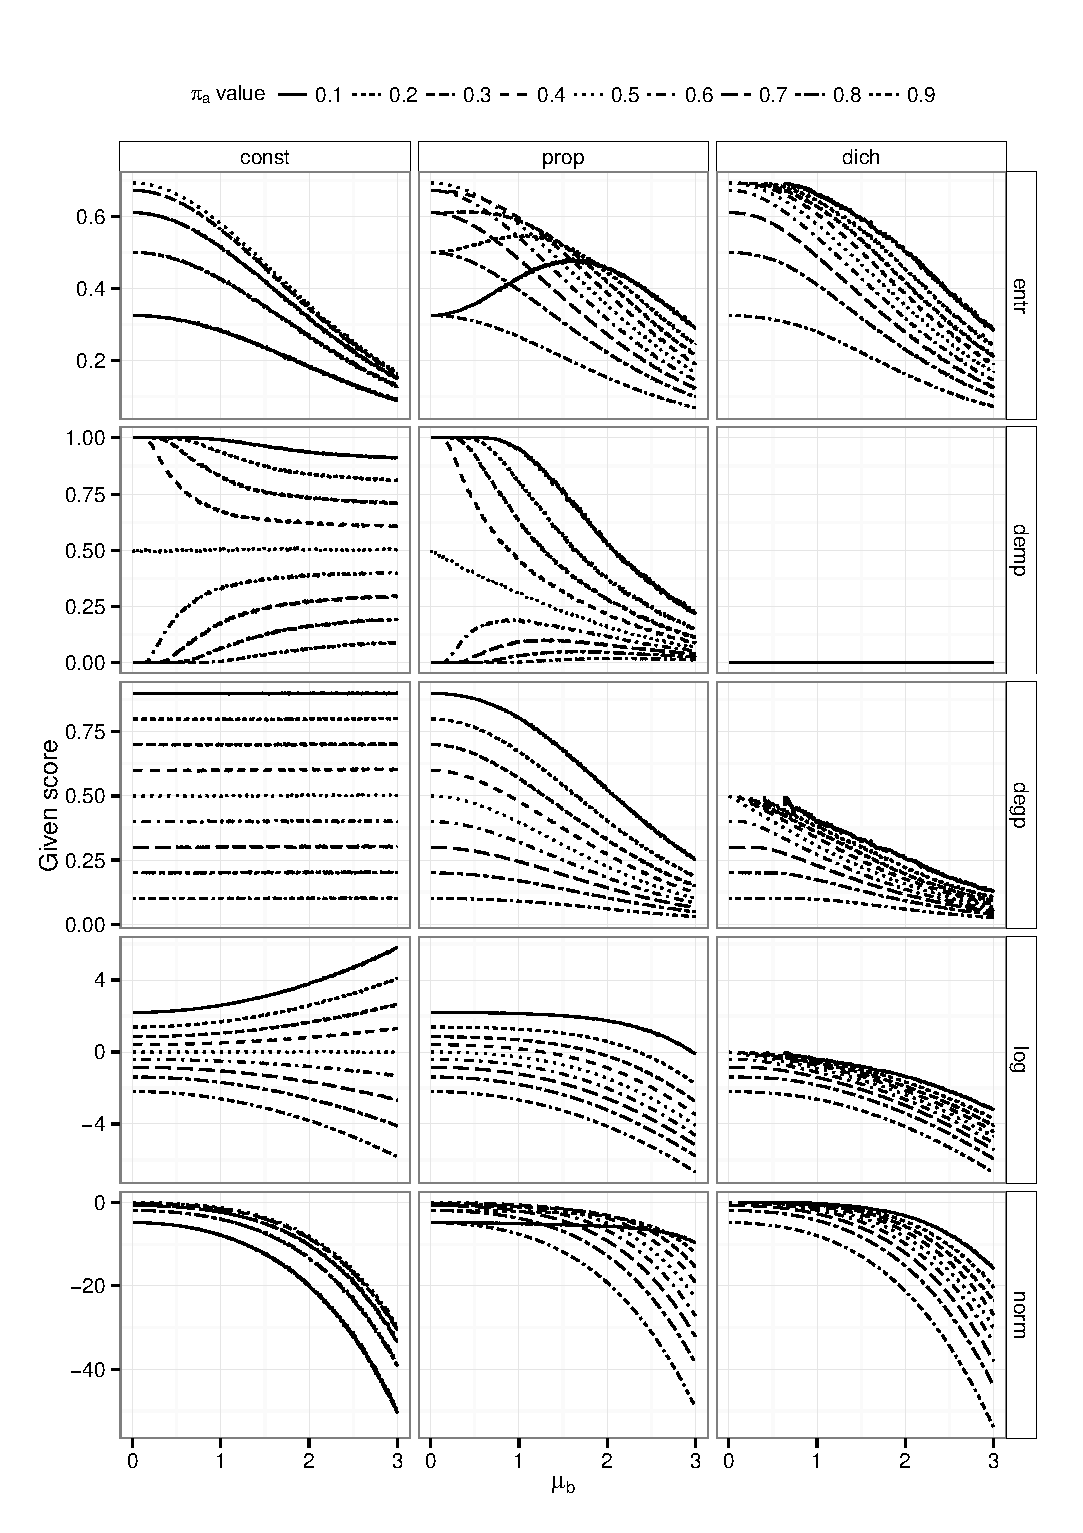
\includegraphics[scale=.5]{fig01all.eps}
\caption{Score calculated for methods described for different approaches of $\lambda$ and $\omega$ score when $\mu_b$ varying}
\label{fig:mu_varying}
\end{figure}

In the first column we have plot the methods for different proposed functions $\lambda$ using the function $\omega(\hat{\m \tau}_{i \mathcal{P}_s}, a) = 1$. In this scenario, only the entropy approach and the norm approach perform as expected, that is, the score decreases as the distance between the centre of distribution $\hat{f}_{I_a}$ and $\hat{f}_{I_b, \mu_b}$ increase. Moreover, for this two methods the obtained score the same when $\pi_a = 1- \pi_a$ {\color{blue} i per tant que les gr\`{a}fiques es solapen}.

In the second column we have plot the methods using the function $\omega(\hat{\m \tau}_{i \mathcal{P}_s}, a) = \hat{\tau}_{iI_a}$. In this case, all the methods perform as expected, the score decreases when $\mu_b$ increases. Note that the entropy and the norm methods become both again symmetric with respect to $\pi_a$ for values of $\mu_b$ close $0$.

In the third column, the score is represented using the function $\omega(\hat{\m \tau}_{i \mathcal{P}_s}, a) = \mathbbm{1}\left( \forall j\; \hat{\tau}_{i I_{a}} \geq \hat{\tau}_{iI_j} \right)$. In this case, all the approaches perform as expected except when $\lambda(\hat{\m \tau}_{i \mathcal{P}_s}, a, b) = \mathbbm{1}\left( \forall j\; \hat{\tau}_{i I_{b}} \geq \hat{\tau}_{iI_j} \right)$. In this case the function is constantly $0$, and therefore it is of no use to decide which components needs to be merged.


To compare, now we include another component keeping the two previous components inside the mixture. Consider the FM
\begin{equation}\label{three_mixture}
f_3 = \pi_a \hat{f}_{I_a} + (0.5 - \pi_a) \hat{f}_{I_b, \mu_b} + 0.5 \hat{f}_{I_c}
\end{equation}
with three components. Component $\hat{f}_{I_a} = N(0, 1)$ is the normal with mean equal to $0$ and variance $1$, component $\hat{f}_{I_b, \mu_b} = N(\mu_b, 1)$ is a normal with mean $\mu_b$ and component $\hat{f}_{I_c} = N(3, 1)$ is the normal with mean equal to $3$ and variance $1$. The two first mixture proportions are parameterised by $\pi_a$ whereas the third one is constantly $0.5$.

Similar to the previous simulation, we have  randomly generated $m=100\;000$ different samples of size $n=500$ from mixture $f_3$. We have evaluated each approach proposed in Table~\ref{table_methods} by varying parameter $\pi_a$ between values $0.05, 0.1, \dots, 0.45$ and parameter $\mu_b$ varying between $0$ and $3$. For each approach and parameter value, we have calculated the mean of the score obtained in each of the $m$ samples. In Figure~\ref{fig:mu_varying3} the obtained means are represented.

\begin{figure}[!t]
\centering
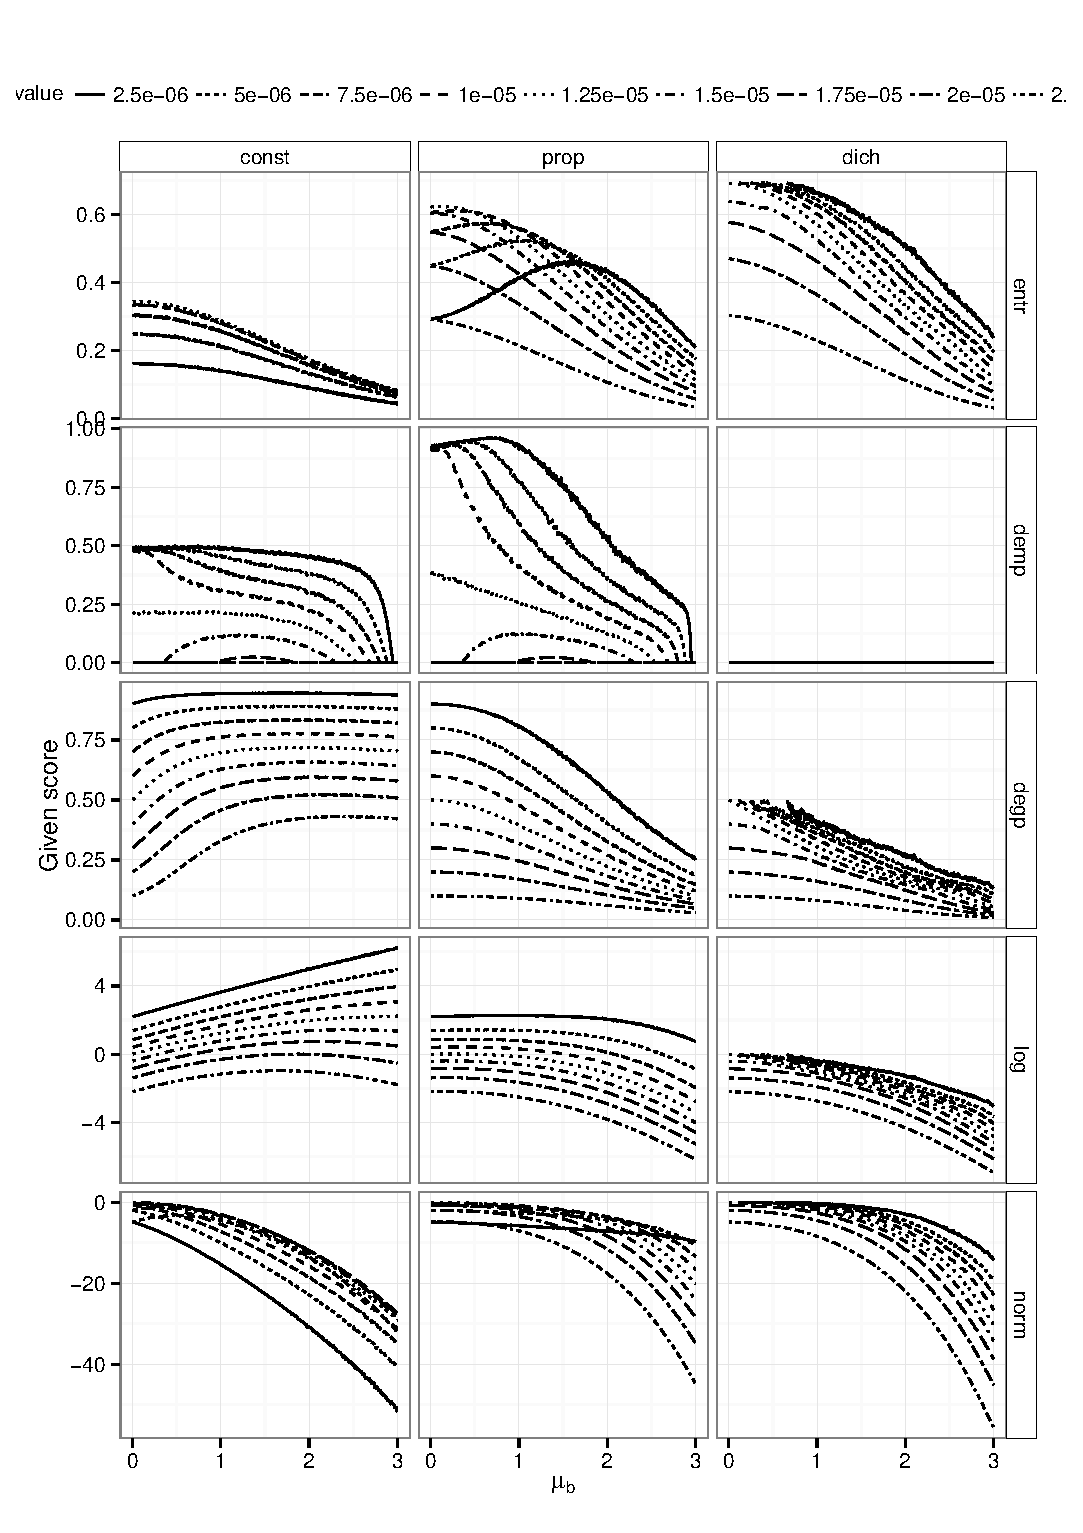
\includegraphics[scale=.5]{fig01ball.eps}
\caption{Score calculated for methods described for different approaches of $\lambda$ and $\omega$ score when $\mu_b$ varying}
\label{fig:mu_varying3}
\end{figure}


Now, the main difference between the results obtained in Figure~\ref{fig:mu_varying} and Figure~\ref{fig:mu_varying3} appear on the first column, which corresponds to those methods with the constant weighing function, i.e. $\omega(\hat{\m \tau}_{i \mathcal{P}_s}, a) = const$. {\color{blue} Alguna explicaci\'{o} de perqu\`{e} passa aix\`{o}?}

In each simulation, the second and third column scores the confusion between components similarly. Note that by construction, when the confusion between part $I_a$ and part $I_b$ is calculated with function $\lambda(\hat{\m \tau}_{i \mathcal{P}_s}, a, b)$, methods $DEGP$, $LOG$ and $LOG^2$ score the same whenever the ratio $\frac{\pi_a}{(1 - \pi_a)}$ and $\frac{\pi_a}{(0.5 - \pi_a)}$ is the same for mixture $f_2$ and $f_3$ respectively.


\subsection{Simulation example}

In this section we have generated different samples to test the performance of methods available at Table~\ref{table_methods}. To simulate our data sets we have used the R package MixSim~\citep{Citar mixxim} {\color{blue} falta la cita!!!}. This package allows us to generate mixtures with a fixed overlapping level, $\hat{\omega}$ {\color{blue} unificar notaci\'{o}. Aqu\'{\i} poses un hat a la omega, a la secci\'{o} 2 o b\'{e} la dones sense hat o b\'{e} amb un check}. The overlapping level $\hat{\omega}$ is a measure of how easy is to confuse two components. In fact,  $\hat{\omega}$ is measured as a probability an therefore it ranges between $0$ and $1$. In Figure~\ref{omega} three different samples coming from three different randomly generated mixtures with overlapping parameters  $\hat{\omega}=0.05$, $\hat{\omega}=0.25$ and $\hat{\omega}=0.45$ are shown.

\begin{figure}[!t]
\centering
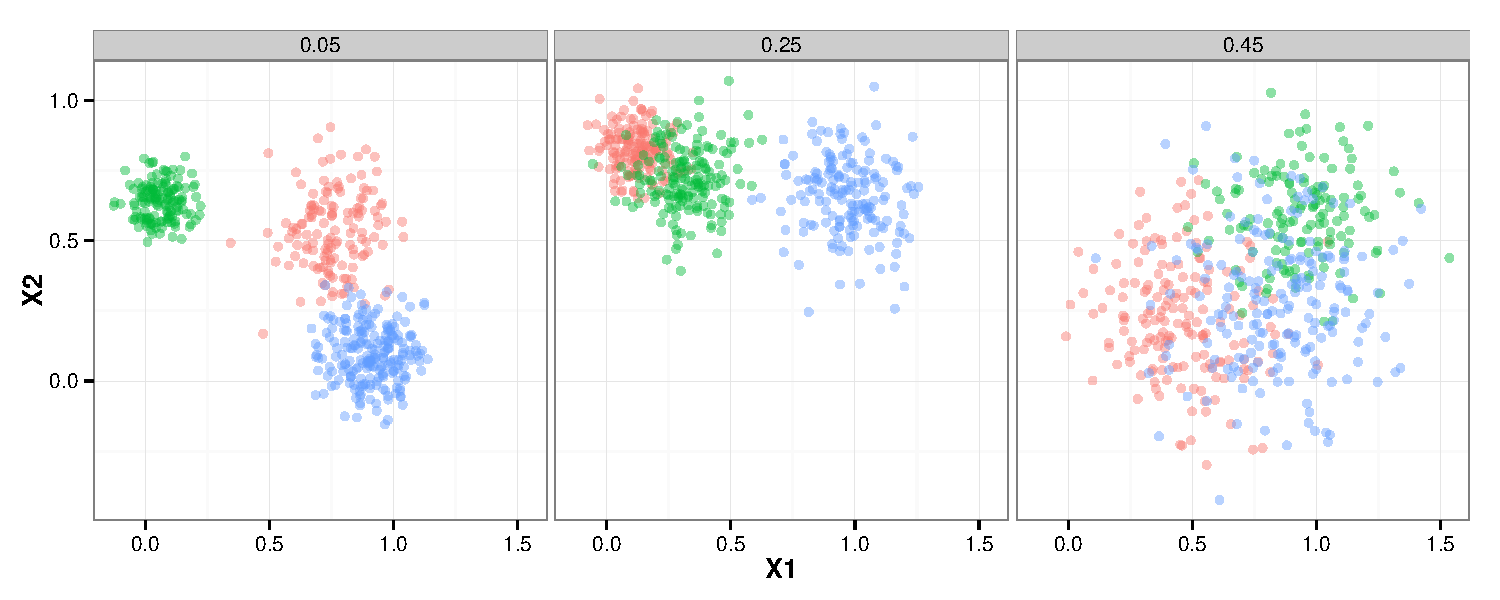
\includegraphics[scale=.5]{omega.pdf}
\caption{Example for different values of parameter $\hat{\omega}$}
\label{omega}
\end{figure}


For different values of $\hat{\omega}$ from $0$ to $0.5$ and each method $\mathcal{M}$ from Table~\ref{table_methods},  we  have repeated $1000$ times the following process:
\begin{enumerate}
\item Generate a sample $X$ of size $n=500$ with $D=5$ coordinates coming from a gaussian mixture with $3$ components whose components have maximum overlapping $\omega$. We keep the component which originates each element of sample $X$. Therefore, we have an original partition to which compare.
\item Fit a mixture with 9 components to sample $X$.
\item Using method $\mathcal{M}$ we have built a hierarchical partition as the one shown in Figure~\ref{hierarchical}.
\item We compare the original partition with the one obtained with method $\mathcal{M}$ at level $3$. To compare the similarity between the original partition and the one obtained in this step, we have used different indices. Because the overall results changed slightly, we have decided to show only one measure of similarity, the Agreement proportion. The Agreement proportion varies between $0$ and $1$, being $1$ a perfect agreement.
\end{enumerate}

Finally, we average the Agreement proportion obtained in the $1000$ simulations.

To compare the performance of presented methods, we have included a method which at step $3$ decides randomly the two components to merge. In Figure~\ref{fig:mub} we have plotted the obtained results. We have separated the methods depending on the weighing function.

In Figure~\ref{fig:mub} left, we have represented the methods which use the constant weighing function $\omega(\hat{\m \tau}_{i \mathcal{P}_s}, a) = const$. For lower levels of overlapping, the Entropy method (\cite{baudry2010combining}) is the one performing better. For higher level of overlapping, the $LOG_2$ and $DEGP$ methods perform slightly better than the others. This is coherent with the graphics shown in Figure~\ref{fig:mu_varying3} where those two methods were the only methods (with constant weighing) decreasing as the distance between distributions increased.

In Figure~\ref{fig:mub} center, we have represented the methods weighing the score by the posterior probability of begin generated by component $\hat{f}_{I_a}$, $\omega(\hat{\m \tau}_{i \mathcal{P}_s}, a) =  \hat{\tau}_{iI_a}$. All methods perform similarly in comparison to the ones which constant weighing function. Between them, the ones with higher agreement proportion are $LOG$ and $LOG^2$ performing almost equally, the one with lower agreement proportion is the $DEMP$ algorithm \citep{hennig2010methods}.

Finally, in Figure~\ref{fig:mub} right, we have represented the methods with dichotomic weighing function. The variation for all those methods is minimum. Remember that, in this case, the $DEMP$ method is of no use.

\section{Conclusions}
\label{conclusions}

\begin{figure}[!h]
\centering
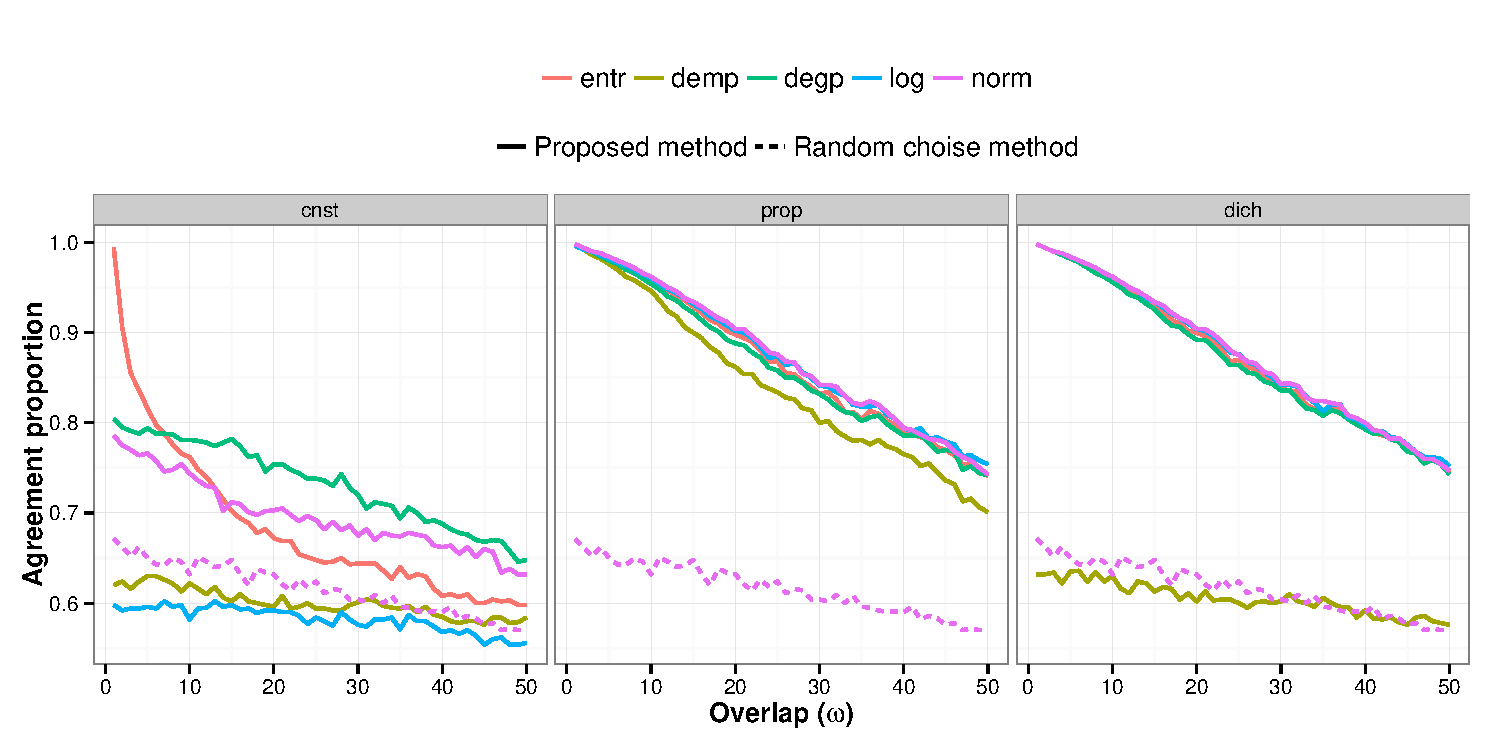
\includegraphics[width=\textwidth]{linesagreement.pdf}
\caption{$\lambda$ Agreement proportion results.}
\label{fig:mub}
\end{figure}


\bibliographystyle{apalike}
\begin{thebibliography}{}

\bibitem[Aitchison, 1986]{aitchison1986statistical}
Aitchison, J. (1986).
\newblock {\em {The Statistical Analysis of Compositional Data}}.
\newblock Monographs on Statistics and Applied Probability. Chapman \& Hall
  Ltd., London (UK).

\bibitem[Aitchison, 2002]{aitchison2002simplicial}
Aitchison, J. (2002).
\newblock {\em {Simplicial inference}}.
\newblock {\em Algebraic Methods in Statistics anb Probability}, 287: 1--22.

\bibitem[Baudry et~al., 2010]{baudry2010combining}
Baudry, J.-P., Raftery, A.~E., Celeux, G., Lo, K., and Gottardo, R. (2010).
\newblock {Combining Mixture Components for Clustering}.

\bibitem[Hennig, 2010]{hennig2010methods}
Hennig, C. (2010).
\newblock {Methods for merging Gaussian mixture components}.
\newblock {\em Advances in Data Analysis and Classification}, 4(1):3--34.

\bibitem[Lee and Cho, 2004]{lee2004combining}
Lee, H.-j. and Cho, S. (2004).
\newblock {Combining Gaussian Mixture Models}.
\newblock In Yang, Z., Yin, H., and Everson, R., editors, {\em Intelligent Data
  Engineering and Automated Learning – IDEAL 2004 SE - 98}, volume 3177 of
  {\em Lecture Notes in Computer Science}, pages 666--671. Springer Berlin
  Heidelberg.

\bibitem[Longford and Bartosova, 2014]{longford2014}
Longford, N.~T. and Bartosova, J. (2014).
\newblock {A confusion index for measuring separation and clustering}.
\newblock {\em Statistical Modelling}, 14(3):229--255.

\bibitem[Melnykov, 2013]{melnykov2013distribution}
Melnykov, V. (2013).
\newblock {On the Distribution of Posterior Probabilities in Finite Mixture
  Models with Application in Clustering}.
\newblock {\em Journal of Multivariate Analysis}, 122:175--189.

\bibitem[Pastore and Tonellato, 2013]{pastore2013merging}
Pastore, A. and Tonellato, S.~F. (2013).
\newblock {A Merging Algorithm for Gaussian Mixture Components}.
\newblock {\em SSRN Electronic Journal}, (04).

\end{thebibliography}

\end{spacing}

\end{document}
